\documentclass[journal]{vgtc}                % final (journal style)
%\documentclass[review,journal]{vgtc}         % review (journal style)
%\documentclass[widereview]{vgtc}             % wide-spaced review
%\documentclass[preprint,journal]{vgtc}       % preprint (journal style)
%\documentclass[electronic,journal]{vgtc}     % electronic version, journal

%% Uncomment one of the lines above depending on where your paper is
%% in the conference process. ``review'' and ``widereview'' are for review
%% submission, ``preprint'' is for pre-publication, and the final version
%% doesn't use a specific qualifier. Further, ``electronic'' includes
%% hyperreferences for more convenient online viewing.

%% Please use one of the ``review'' options in combination with the
%% assigned online id (see below) ONLY if your paper uses a double blind
%% review process. Some conferences, like IEEE Vis and InfoVis, have NOT
%% in the past.

%% Please note that the use of figures other than the optional teaser is not permitted on the first page
%% of the journal version.  Figures should begin on the second page and be
%% in CMYK or Grey scale format, otherwise, color shifting may occur
%% during the printing process.  Papers submitted with figures other than the optional teaser on the
%% first page will be refused.

%% These three lines bring in essential packages: ``mathptmx'' for Type 1
%% typefaces, ``graphicx'' for inclusion of EPS figures. and ``times''
%% for proper handling of the times font family.

\usepackage{mathptmx}
\usepackage{graphicx}
\usepackage{times}
\usepackage{balance}
\usepackage[nooneline,hang,it,IT]{subfigure}

%% We encourage the use of mathptmx for consistent usage of times font
%% throughout the proceedings. However, if you encounter conflicts
%% with other math-related packages, you may want to disable it.

%% This turns references into clickable hyperlinks.
\usepackage[bookmarks,backref=true,linkcolor=black]{hyperref} %,colorlinks
\hypersetup{
  pdfauthor = {},
  pdftitle = {},
  pdfsubject = {},
  pdfkeywords = {},
  colorlinks=true,
  linkcolor= black,
  citecolor= black,
  pageanchor=true,
  urlcolor = black,
  plainpages = false,
  linktocpage
}

%% If you are submitting a paper to a conference for review with a double
%% blind reviewing process, please replace the value ``0'' below with your
%% OnlineID. Otherwise, you may safely leave it at ``0''.
\onlineid{0}

%% declare the category of your paper, only shown in review mode
\vgtccategory{Research}

%% allow for this line if you want the electronic option to work properly
\vgtcinsertpkg

%% In preprint mode you may define your own headline.
%\preprinttext{To appear in an IEEE VGTC sponsored conference.}

%% Paper title.

\title{AiPoker - Implementation of a Poker Agent}

%% This is how authors are specified in the journal style

%% indicate IEEE Member or Student Member in form indicated below
\author{John Holl\'en, Robin Berntsson, Simon Bergst\"om}
\authorfooter{
%% insert punctuation at end of each item
\item
 John Holl\'en, Robin Berntsson, Simon Bergstr\"om
}

%% Abstract section.
\abstract{ 
We will probably write this section the last thing we do. 
}
%% Keywords that describe your work. Will show as 'Index Terms' in journal
%% please capitalize first letter and insert punctuation after last keyword
\keywords{Monte Carlo Tree Search, Texas Hold'em}



%%%%%%%%%%%%%%%%%%%%%%%%%%%%%%%%%%%%%%%%%%%%%%%%%%%%%%%%%%%%%%%%
%%%%%%%%%%%%%%%%%%%%%% START OF THE PAPER %%%%%%%%%%%%%%%%%%%%%%
%%%%%%%%%%%%%%%%%%%%%%%%%%%%%%%%%%%%%%%%%%%%%%%%%%%%%%%%%%%%%%%%%

\begin{document}

%% The ``\maketitle'' command must be the first command after the
%% ``\begin{document}'' command. It prepares and prints the title block.

%% the only exception to this rule is the \firstsection command
\firstsection{Background}
\maketitle 
Texas Hold'em is a popular variant of poker, not just to play with friends but also online against other people for money. Poker belongs with the most difficult kind of card game to solve discretely since it is an stochastic game with imperfect information. The challenge of creating the best poker agent has attracted a lot of people and is a popular subject in AI development.

The theory behind Monte Carlo search trees will be studied within this project and tested as a part of the logic that will determine the actions of the poker agent. Smaller algorithms to improve the logic for the AI will be tested and implemented in combination of the Monte Carlo Search Tree to create the best possible poker agent.

\section{Theory}
\subsection{Characteristics of a Poker Player}
Like previously described poker is a stochastic game, that makes it very hard to control and to define what a good poker player is. A good poker player does not always need to be the one who is a winning player. But in this project a aim has been set to try to create a poker agent who wants to win and will not take too much risk when playing. But to not make the agent to predictable the agent shall randomly switch behavior between aggressive and passive playing. 

\section{Method}
\subsection{Basic Game Engine}
In order to even begin implementing an AI, the core poker game had to be implemented first. For simplicity the game implemented in this study is a two player game where a human player faces a computer AI. The player who starts is chosen at random when the game is started. The player that starts then puts one dollar in to the pot. The other player puts two dollars in the pot. Then the game is turn based like ordinary Texas Hold?em, the players can bet, check, call, raise and fold. And after each betting round cards are dealt to the table and the players combine the cards on hand with the cards on the table in order to get the strongest hand possible. 

To be able to test the game engine the computer was first set to do moves completely at random. When all this was done the implementation of the AI could start.

\subsection{AI - techniques}
\subsubsection{Monte Carlo Tree Search}
MCTS is a best-first search strategy. Every node in the tree contain two values, an estimate of the expected value $V(P)$ of the reward $r(P)$ and the number of times the node have been visited $n_{i}$. MCTS only starts with the root node and incrementally build the tree by repeating the following 4 steps.\\*\\*
\textbf{Selection}
\\*Selection is made by starting from the root node and then recursively select nodes until a leaf node is reached (this does not have to be a leaf of the game tree). To determine which node is the optimal one, the upper confidence bounds (UCB1) formula is used: 

\begin{equation} \label{eq:upperconfidence}
	v_{i} + C \cdot \sqrt{\frac{\ln N}{n_{i}}}
\end{equation}
The first term vi is the estimated value of the node and is responsible for exploitation of good nodes, the second term is made up by the total number of visits of the parent node $N$ and the total number of visits of the current node $n_{i}$. The constant $C$ allows tuning of the exploration-exploitation trade-off. 
\\*\\*
\textbf{Expansion}
\\*If the leaf node reached is not an terminating node, which means that the game is not over at the current node. Then create one or more child nodes from the node currently at. This step is illustrated in fig(\ref{fig:expansion}).
\begin{figure}[here]
  \begin{center}
    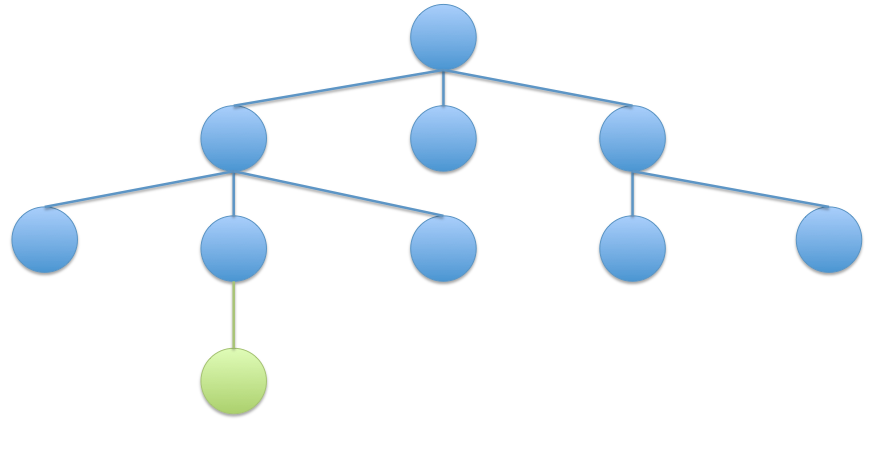
\includegraphics[scale=0.30]{img/tree1.png}
    \caption{\label{fig:expansion} Illustration of how the green node is added to the tree.}
  \end{center}
\end{figure}
\\*
\textbf{Simulation}
\\*The third step in MCTS is the simulation step. Here a game is simulated from the state in the new node until a result is achieved. The value of the reached result is recorded.
\\*\\*
\textbf{Backpropagation}
\\*The last step is to update the expected value and the selection counter for all nodes along the explored path by backpropagating the recorded result from the simulation step. This step is illustrated in fig(\ref{fig:backprop}).
\begin{figure}[here]
  \begin{center}
    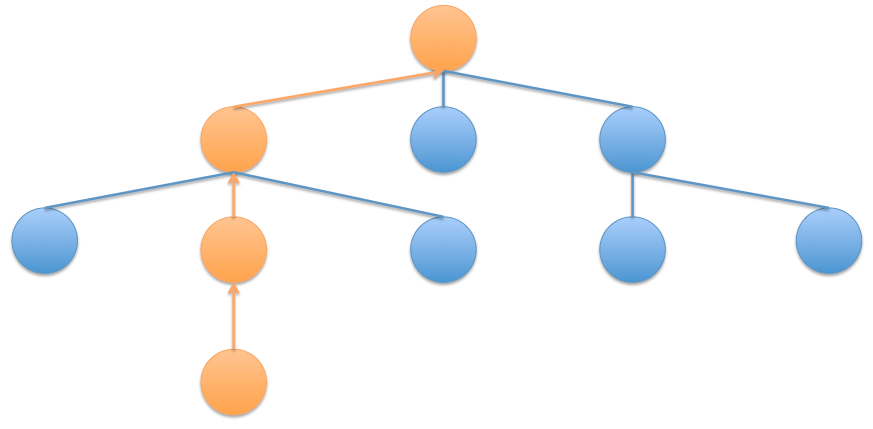
\includegraphics[scale=0.30]{img/tree2.png}
    \caption{\label{fig:backprop} Illustration of how the path to the node is updated with the score from the simulation in the whole tree.}
  \end{center}
\end{figure}
When the back propagation step is finished the whole chain starts over again starting with the selection step. This is done until the either the game tree is fully searched or a time limit is reached. The fact that MCTS can give a result after a given time is a result of it being anytime, that is it will give a valid solution to the problem even if it is interrupted before it is finished. However the quality of the solution is an estimate and is expected to be better the more time the MCTS keeps running.

One problem that is introduced with the MCTS is how to run the simulation step. Here we have to select the moves for each player until the end of the game. One solution could be to just select random moves, this can work well for simple games but for games as complex as poker this will lead to bad results. This implies that we somehow have to model the opponent to be able to determine the correct actions in the simulation.  

\subsubsection{Hand Strength}
Since Monte Carlo is a heuristic search which simulate a set of outcomes in a game to calculate what action to make the logic so far does not consider how good  the cards on the agents hand is compared to other hands. To add this logic to the agent an algorithm could be used that would return a probability of how strong the current hand cards is with the cards on the table. This probability of the Hand Strength may, at the earliest be calculated the the flop has been shown. [REF!]

The Hand Strength is calculated by comparing the cards on the hand with all possible combination of two cards that the opponent can have and sum the time the agents cards wins compared to the opponent and divide by the number of combinations that was simulated.

\subsubsection{Hand Potential}
The hand potential algorithm calculates the quality of the hand as the game goes on. The algorithm is similar to the hand strength algorithm. The difference is that the hand potential algorithm considers all possible cards that have not been revealed yet. It is also heavier to calculate since it has to go through every possible combination of cards that could possibly end up on the table. It also takes into account every possible card the opponent might have on hand.

\subsubsection{Effective Hand Strength}
By combining the hand strength with the hand potential a probability of winning can be calculated, and this is called the effective hand strength and is calculated as following:

\begin{equation} \label{EHS}
	EHS = HS \cdot (1-NPot) \cdot PPOT
\end{equation}

\subsection{Implementation}
\subsubsection{Main Design}
The application implemented in this study was implemented in Javascript using the library Three.js for visualization. Three.js is a webGL library which provides high level functions for creating a 3D scene.

The application is implemented in an object oriented manner. The main application file is called main.js and it is here the scene is created and where all the other classes needed are initialized. The file main.js also contains all the click listeners for the buttons the human player uses to do moves. An overview over the game architecture is shown in fig(\ref{fig:arcitect}). 
\begin{figure}[here]
  \begin{center}
    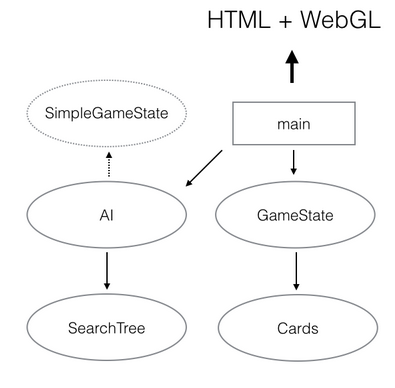
\includegraphics[scale=0.50]{img/arcitect.png}
    \caption{\label{fig:arcitect} Illustration of how the path to the node is updated with the score from the simulation in the whole tree.}
  \end{center}
\end{figure}

\subsubsection{Game}
The main.js file is first painting the poker table and all buttons on the page, when you click the start button a GameState object and a AI will be created.
The poker game is originated from the GameState object which only consists of a Cards object and functions for every state of the poker game Texas Hold'em. The game is created for two players where one player is an AI agent and the other player is the client controlled by a human. The Cards object consist of a full deck of cards and all methods needed for playing Texas Hold?em like shuffle the deck of cards, deliver the flop, turn card, river card and cards for the players.

\section{Result}
\subsection{The Game}
The result of this study is a Texas Hold'em game with an AI implemented using several different AI techniques and combining them together. The game is fully playable with an opponent that is somewhat realistic in the way it chooses what move to make. The 3D-scene is used to visualise the poker table, and it also shows the cards on hand. This is shown in fig(\ref{fig:3dscene}).
\begin{figure}[here]
  \begin{center}
    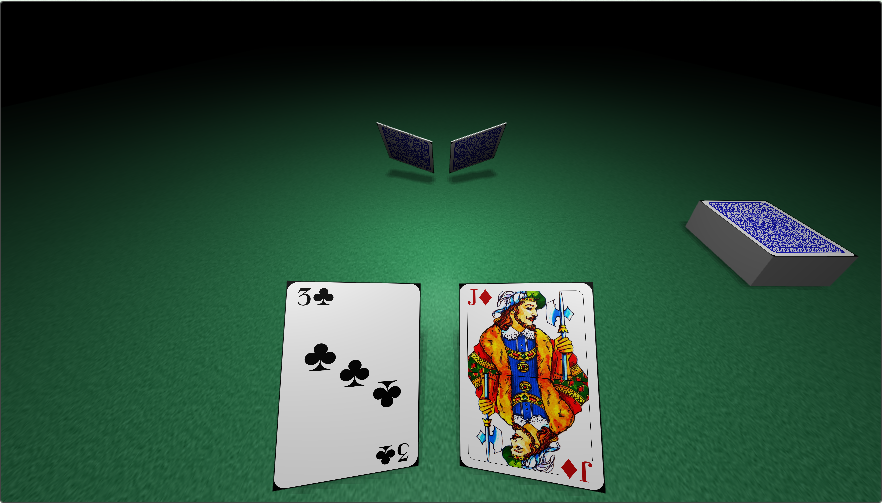
\includegraphics[scale=0.30]{img/3dscene.png}
    \caption{\label{fig:3dscene} The 3D-scene in the final version showing the player's cards on hand.}
  \end{center}
\end{figure}

To the left of the 3D-scene there are some additional UI-elements. these are the buttons telling the player what moves he or she can make. By pressing one of these buttons the player will make a move. The coloured buttons indicate that a move is valid. The greyed out buttons indicate invalid moves. The buttons are shown in fig(\ref{fig:ui1}).
\begin{figure}[here]
  \begin{center}
    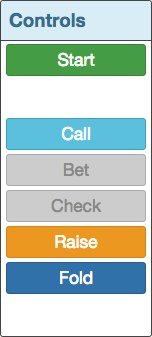
\includegraphics[scale=0.50]{img/ui1.png}
    \caption{\label{fig:ui1} The player controls, placed to the left of the 3D-scene.}
  \end{center}
\end{figure}

To the right of the 3D-scene some information is shown. Information about money is shown in the upper box. How much money each player has, and how much money there is currently on the table. This information box is illustrated in fig(\ref{fig:ui2}).
\begin{figure}[here]
  \begin{center}
    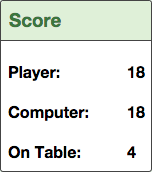
\includegraphics[scale=0.50]{img/ui2.png}
    \caption{\label{fig:ui2} The score board giving the player information about the money currently in play.}
  \end{center}
\end{figure}

Right below the score board, the enemy log is placed. It keeps track of what the computer does each time it makes a move. Since this is quite hard to visualise the decision was made to print the computer's move in text every time it makes a move. The enemy log is shown in fig(\ref{fig:ui3}).
\begin{figure}[here]
  \begin{center}
    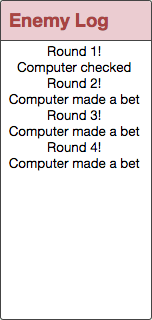
\includegraphics[scale=0.50]{img/ui4.png}
    \caption{\label{fig:ui3} The enemy log, showing what the computer has done each round.}
  \end{center}
\end{figure}

\subsection{AI}
Since a number of algorithms were implemented in this study several results were achieved and therefore comparisons between the different approaches can be made. 

\section{Conclusion}



\begin{thebibliography}{9}

\bibitem{byron}
  Byron L., Wattenberg M.
  \emph{Stacked graphs - Geometry \& Aesthetics}.
  IEEE Transactions on Visualization and Computer Graphics archive
Volume 14 Issue 6,
Pages 1245-1252. IEEE Educational Activities Department Piscataway, NJ, USA
ISSN: 1077-2626.
  2008.

\bibitem{reynolds}
  Reynolds A. P., Richards G., Rayward-Smith V. J.
  \emph{The Application of K-medoids and PAM to the Clustering of Rules}.
  In: Intelligent Data Engineering and Automated Learning - IDEAL 2004. Lecture Notes in Computer Science, 3177 . Springer-Verlag, pp. 173-178. ISBN 978-3-540-22881-3,
  2004.

\end{thebibliography}

\end{document}
